% Copyright (C) 2020 Diogo Rodrigues, Breno Pimentel
% Distributed under the terms of the GNU General Public License, version 3

\documentclass[a4paper, 11pt]{report}
\usepackage[top=35mm,bottom=35mm,left=25mm,right=25mm]{geometry} % Margins

% Change section numbers
\renewcommand{\thesection}{\arabic{section}}

% Second page
\usepackage{secondpage}
\usepackage{datetime}

% Appendix
\usepackage{appendix}

% Landscape pages
\usepackage{pdflscape}
\usepackage{multicol}
\setlength\columnsep{50pt}

% Decent underlines
\usepackage[normalem]{ulem}

% Hyper-references
\usepackage{hyperref}

% Imports
\usepackage{import}

% Graphics and images
\usepackage{graphicx} \graphicspath{{./images/}}
\usepackage{tikz}
\usepackage{tikz-qtree}
\usetikzlibrary{automata, positioning, shapes, arrows}
\usepackage[justification=centering,font=small,skip=0.5em]{caption}
\usepackage{subcaption}
\usepackage{float}

\usepackage[binary-units=true]{siunitx} %SI units
\usepackage{pgfplots}
\pgfplotsset{compat=newest} % Allows to place the legend below plot
\usepgfplotslibrary{units} % Allows to enter the units nicely
\sisetup{
  round-mode          = places,
  round-precision     = 2,
}

% Encodings (to render letters with diacritics and special characters)
\usepackage[utf8]{inputenc}
% \DeclareUnicodeCharacter{2192}{\dash}

% Language
\usepackage[english]{babel}

% Source code and algorithms
%\usepackage{amsmath}
\usepackage{algorithm}
\usepackage[noend]{algpseudocode}
\usepackage{listings, chngcntr}
\lstset{
	basicstyle=\linespread{0.85}\ttfamily,
	basewidth  = {0.50em,1em},
    frame=tbr, % draw frame at top and bottom of the code
    tabsize=4, % tab space width
    numbers=left, % display line numbers on the left
	showstringspaces=false, % don't mark spaces in strings    
    commentstyle=\color{green}, % comment color
    keywordstyle=\color{blue}, % keyword color
    stringstyle=\color{red}, % string color
    breaklines=true,
    postbreak=\mbox{\textcolor{red}{$\hookrightarrow$}\space}
}
\lstdefinelanguage{cisco}{
    keywords = {
        enable,
        copy, reload,
        configure, terminal, end, interface, switchport, mode,
        access, vlan, show, interfaces, ip, address,
        no, shutdown, exit, nat, inside, outside, route, list, permit,
        pool, source, ovrld, overload, running, id
    },
    morecomment = [l]{\#}
}


% Tables with bold rows
\usepackage{tabularx}
\newcommand\setrow[1]{\gdef\rowmac{#1}#1\ignorespaces}
\newcommand\clearrow{\global\let\rowmac\relax}
\clearrow
\usepackage{multirow}

% Tables with vertical center alignment
\usepackage{array}

% Lists and items
\usepackage{enumitem}

% Math stuff
\usepackage[mathscr]{euscript}
\usepackage{amssymb, latexsym} %Load math symbols like \blacksquare, but also load normal \leadsto arrows
\usepackage{mathtools} % For \text{...}
% \usepackage{enumitem}
% \usepackage{xcolor}
\newcommand{\expnumber}[2]{{#1}\mathrm{e}{#2}} % scientific notation
\newcommand{\degree}{^{\circ}}
\newcommand*\xor{\oplus}
\newcommand\expected[1]{\mathbf{E}[#1]}

% Headers and footers
\usepackage{fancyhdr}
\pagestyle{fancyplain}
\fancyhf{}
\lhead{\fancyplain{}{Configuration of a computer network — Report (RCOM 2020/21)}}
\rhead{\fancyplain{}{Class 2, group 4}}
\lfoot{\fancyplain{}{\leftmark}}
\rfoot{\thepage}

% Email
\newcommand{\email}[1]{
{\texttt{\href{mailto:#1}{#1}} }
}

% Metadata
\title{\Huge Configuration and study of a \\ computer network \\ \vspace*{12pt} \Large Report \\ \vspace*{4pt} \large FEUP - RCOM 2020/21}
\author{
Class 2, group 4 \vspace{0.5em} \\
\begin{tabular}{r l}
	\email{up201800170@fe.up.pt} & Breno Accioly de Barros Pimentel \\
	\email{up201806429@fe.up.pt} & Diogo Miguel Ferreira Rodrigues  \\
\end{tabular}
}
\date{23rd of December, 2020}

% Document
\begin{document}
\maketitle
\begin{secondpage}
    Copyright \copyright 2020--\the\year\ Diogo Rodrigues, Breno Pimentel\par
    \IfFileExists{VERSION}{Version \input{VERSION}}{Draft version}\par
    \immediate\write18{./get-commit-info.sh > COMMIT.tex}
    Built on \today~\currenttime~from \href{https://github.com/dmfrodrigues/feup-rcom-l2}{dmfrodrigues/feup-rcom-l2}, commit \input{COMMIT}\unskip.\par
    Permission is granted to copy and distribute this document under the terms of the
    \href{https://creativecommons.org/licenses/by-nc-nd/4.0/}{Creative Commons Attribution-NonCommercial-NoDerivatives 4.0 International}
    public license.
\end{secondpage}
\clearpage

\pagenumbering{arabic}

\section*{Summary}

This project was elaborated as the second project in the context of the curricular unit Computer Networks (RCOM), part of the Integrated Master in Informatics and Computing Engineering (MIEIC) at the Faculty of Engineering of the University of Porto (FEUP).
It concerns the configuration of a computer network, and its test and study through a developed FTP client.

All objectives were fulfilled, as we successfully implemented in C a simple FTP client for file retrieval over the Internet, and the configured network abided to the guidelines' requirements.

\section*{Introduction} \label{sec:Introduction}

The present project aims at developing a simple FTP client which is to be tested over a configured network.
The source code was developed in the C language, targeting Linux devices.
The goal network is composed of three computers, a switch that implements two virtual sub-networks, and a router to provide Internet access.

This report describes the corresponding project's activities, and is divided into two parts.
In part 1 we address the design, development and testing of the FTP client.
In part 2 we describe the steps on configuring the computer network, over the course of seven short experiments that incrementally contribute to the final network configuration.
This project was tested in the computers of FEUP, room I321, bench 3, with rack computers 2, 3 and 4, a Cisco Catalyst 3560 Series switch and a Cisco 2900 Series router.

\section{Download application} \label{sec:Part1}

A simple FTP client was developed to test the network configuration.

\subsection{Application architecture} \label{sec:Arc}

The application first parses and verifies if the URL abides to \cite{rfc1738} using a regular expression (\texttt{ftp://[<user>:<password>@]<host>/<url-path>}).
Then it finds the IP address with a call to \texttt{gethostbyname} and the application opens a connection using a socket through port 21 to the FTP server. 

After connecting, it logs in to the server, or otherwise logs in as anonymous if no credentials were provided.
Next, it sends a \texttt{PASV} command to the FTP server so it can transfer data in passive mode; if successful, the server will reply
with six bytes, the first four being the server IP address it just opened for transfer, and the other two the port the server is listening on. 

After entering passive mode, the download application opens another socket, using the port provided by the server, where the data will be transferred.
Finally, it copies the file from \texttt{<url-path>} to the current working directory and finishes the connection by sending the \texttt{QUIT} command and closing the sockets.

To build the application, run \texttt{make} in directory \texttt{download}. To test the application, run:

\begin{lstlisting}[frame=none, numbers=none, language=sh]
./download ftp://[<user>:<password>@]<host>/<url-path>
\end{lstlisting}


\subsection{Report of successful download} \label{sec:Dow}

The application was tested in different FTP servers, with files varying in size and type, with and without credentials.
Reports can be found in \ref{listing:6-2-tux33-pipe}, \ref{listing:6-2-tux33-pic2}, \ref{listing:6-5-tux32} and \ref{listing:6-5-tux33}.

\section{Network configuration and analysis} \label{sec:Part2}

\subsection{Experiment 1} \label{sec:Exp1}

\begin{figure}[H]
	\centering
    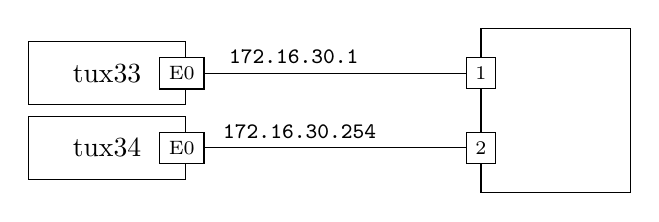
\begin{tikzpicture}[-,>=stealth',node distance=2cm,initial text=$ $,scale=0.95]
        \node at (0,-0) [rectangle,draw,minimum height=0.8cm, minimum width=2cm] (tux33) {tux33};
        \node at (1.0, -0) [rectangle, draw, fill=white] (tux33_E0){ \scriptsize E0 };

        \node at (0,-1.0) [rectangle,draw, minimum height=0.8cm, minimum width=2cm] (tux34) {tux34};
        \node at (1.0, -1) [rectangle, draw, fill=white] (tux34_E0){ \scriptsize E0 };
        


        \draw   (5, +0.6) rectangle ++(2, -2.2);
        \node at (5.0, -0.00) [rectangle, draw, fill=white] (switch_1){ \scriptsize 1 };
        \node at (5.0, -1.00) [rectangle, draw, fill=white] (switch_2){ \scriptsize 2 };

        \draw   (tux33_E0)    edge[above, align=left]     node[xshift=-0.45cm]{\footnotesize \texttt{172.16.30.1  }}          (switch_1)
                (tux34_E0)    edge[above, align=left]     node[xshift=-0.45cm]{\footnotesize \texttt{172.16.30.254}}          (switch_2)
            ;
    \end{tikzpicture}
	\caption{Network architecture for experiment 1}
	\label{fig:network_exp1}
\end{figure}

\subsubsection{Objectives} \label{sec:Obj1}

\begin{enumerate}
    \item Connect two computers by configuring their IP addresses.
\end{enumerate}

\subsubsection{Main configuration commands} \label{sec:Com1}

\begin{tabular}{l | p{75mm} | l}
    \textbf{Dev.} & \textbf{Description}                                  & \textbf{Commands}                       \\ \hline
    tux33         & Activate \texttt{eth0} interface                     & \texttt{ifconfig eth0 up}               \\
    tux33         & Set \texttt{eth0} IP 172.16.30.1, with 24-bit mask   & \texttt{ifconfig eth0 172.16.30.1/24}   \\ \hline
    tux34         & Activate \texttt{eth0} interface                     & \texttt{ifconfig eth0 up}               \\
    tux34         & Set \texttt{eth0} IP 172.16.30.254, with 24-bit mask & \texttt{ifconfig eth0 172.16.30.254/24} \\
\end{tabular}

\subsubsection{Logs analysis} \label{sec:Log1}

ARP is used to map an IP address to a MAC address.
Before sending a frame, the computer first needs to know the MAC address of the receiver.
If the emitter does not have an entry with the receiver IP in its ARP table, it will broadcast a ARP packet with the receiver IP and wait for its response.
As seen in the logs, ARP broadcasts a request for the desired IP address 172.16.30.254 (tux34).
Then tux34 identifies itself, sending another ARP packet with its MAC address 00:21:5a:5a:7d:74.

The ping command generates ICMP (Internet Control Message Protocol) packets. The MAC and IP addresses of the ping packets are the source addresses MAC: 00:21:5a:61:24:92 IP: 172.16.30.1
and destination addresses MAC: 00:21:5a:7d:74 IP: 172.16.30.254.

It is possible to determine if a receiving Ethernet frame is ICMP by checking its IPv4 field and verifying the value 0x01 in the protocol byte.
A ARP frame can be identified with the type value 0x806 in the Ethernet II layer. We could also determine the length of a receiving frame by adding all the frame bytes.

The loopback interface is used by the computer to send and receive packets to itself.
In the experiment, we could verify loopback packets every 10 seconds when the source and destination addresses were equal.
It is important for diagnostics.


\subsection{Experiment 2} \label{sec:Exp2}

\begin{figure}[H]
	\centering
    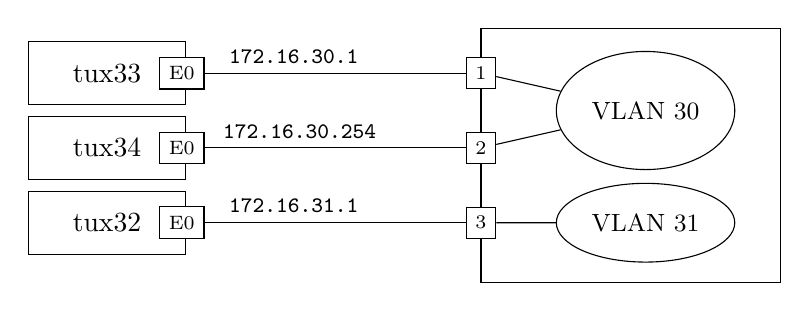
\begin{tikzpicture}[-,>=stealth',node distance=2cm,initial text=$ $,scale=0.95]
        \node at (0,-0) [rectangle,draw,minimum height=0.8cm, minimum width=2cm] (tux33) {tux33};
        \node at (1.0, -0) [rectangle, draw, fill=white] (tux33_E0){ \scriptsize E0 };

        \node at (0,-1.0) [rectangle,draw, minimum height=0.8cm, minimum width=2cm] (tux34) {tux34};
        \node at (1.0, -1) [rectangle, draw, fill=white] (tux34_E0){ \scriptsize E0 };
        
        \node at (0,-2) [rectangle,draw, minimum height=0.8cm, minimum width=2cm] (tux32) {tux32};
        \node at (1.0, -2) [rectangle, draw, fill=white] (tux32_E0){ \scriptsize E0 };

        \draw   (5, +0.6) rectangle ++(4, -3.4);
        \node at (7.2, -0.5) [ellipse, draw, minimum height = 1.5cm, minimum width = 2.0cm, align=center] (VLAN30) {\small VLAN 30};
        \node at (7.2, -2.0) [ellipse, draw, minimum height = 1.0cm, minimum width = 2.0cm, align=center] (VLAN31) {\small VLAN 31};
        \node at (5.0, -0.00) [rectangle, draw, fill=white] (switch_1){ \scriptsize 1 };
        \node at (5.0, -1.00) [rectangle, draw, fill=white] (switch_2){ \scriptsize 2 };
        \node at (5.0, -2.00) [rectangle, draw, fill=white] (switch_3){ \scriptsize 3 };

        \draw   (tux33_E0)    edge[above, align=left]     node[xshift=-0.45cm]{\footnotesize \texttt{172.16.30.1  }}          (switch_1)
                (tux34_E0)    edge[above, align=left]     node[xshift=-0.45cm]{\footnotesize \texttt{172.16.30.254}}          (switch_2)
                (tux32_E0)    edge[above, align=left]     node[xshift=-0.45cm]{\footnotesize \texttt{172.16.31.1  }}          (switch_3)
                
                (switch_1) edge[] (VLAN30)
                (switch_2) edge[] (VLAN30)
                (switch_3) edge[] (VLAN31)
            ;

    \end{tikzpicture}
	\caption{Network architecture for experiment 2}
	\label{fig:network_exp2}
\end{figure}

\subsubsection{Objectives} \label{sec:Obj2}

\begin{enumerate}
    \item Create virtual LAN 30 and add tux33 and tux34 to it.
    \item Create virtual LAN 31 and add tux23 to it.
\end{enumerate}

\subsubsection{Main configuration commands} \label{sec:Com2}

\begin{tabular}{l | p{75mm} | l}
    \textbf{Dev.} & \textbf{Description}                                  & \textbf{Commands}                       \\ \hline
    switch        & Create virtual LAN 30                                 &
        \begin{lstlisting}[frame=none, numbers=none, language=sh]
configure terminal
vlan 30
end
        \end{lstlisting} \\
    switch        & Assign port 1 to VLAN 30                              & 
        \begin{lstlisting}[frame=none, numbers=none, language=sh]
configure terminal
interface fastethernet 0/1
switchport mode access
switchport access vlan 30
end
        \end{lstlisting} \\
\end{tabular}

\subsubsection{Logs analysis} \label{sec:Log2}

There are two broadcast domains, 172.16.31.255 and 172.16.30.255.

\subsection{Experiment 3} \label{sec:Exp3}

\begin{figure}[H]
	\centering
    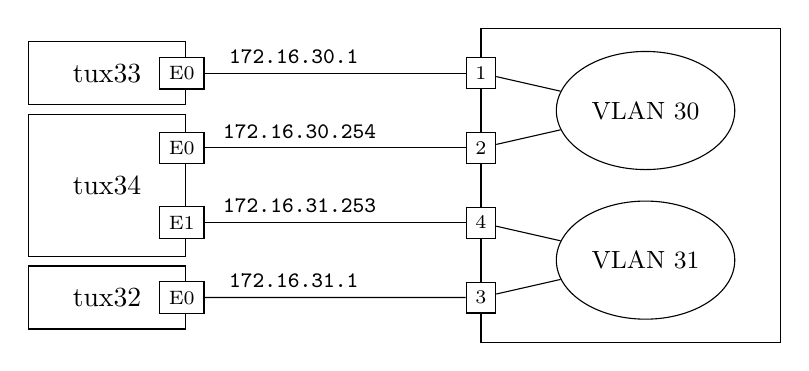
\begin{tikzpicture}[-,>=stealth',node distance=2cm,initial text=$ $,scale=0.95]
        \node at (0,-0) [rectangle,draw,minimum height=0.8cm, minimum width=2cm] (tux33) {tux33};
        \node at (1.0, -0) [rectangle, draw, fill=white] (tux33_E0){ \scriptsize E0 };

        \node at (0,-1.5) [rectangle,draw, minimum height=1.8cm, minimum width=2cm] (tux34) {tux34};
        \node at (1.0, -1) [rectangle, draw, fill=white] (tux34_E0){ \scriptsize E0 };
        \node at (1.0, -2) [rectangle, draw, fill=white] (tux34_E1){ \scriptsize E1 };
        
        \node at (0,-3) [rectangle,draw, minimum height=0.8cm, minimum width=2cm] (tux32) {tux32};
        \node at (1.0, -3) [rectangle, draw, fill=white] (tux32_E0){ \scriptsize E0 };

        \draw   (5, +0.6) rectangle ++(4, -4.2);
        \node at (7.2, -0.5) [ellipse, draw, minimum height = 1.5cm, minimum width = 2.0cm, align=center] (VLAN30) {\small VLAN 30};
        \node at (7.2, -2.5) [ellipse, draw, minimum height = 1.5cm, minimum width = 2.0cm, align=center] (VLAN31) {\small VLAN 31};
        \node at (5.0, -0.00) [rectangle, draw, fill=white] (switch_1){ \scriptsize 1 };
        \node at (5.0, -1.00) [rectangle, draw, fill=white] (switch_2){ \scriptsize 2 };
        \node at (5.0, -2.00) [rectangle, draw, fill=white] (switch_4){ \scriptsize 4 };
        \node at (5.0, -3.00) [rectangle, draw, fill=white] (switch_3){ \scriptsize 3 };

        \draw   (tux33_E0)    edge[above, align=left]     node[xshift=-0.45cm]{\footnotesize \texttt{172.16.30.1  }}          (switch_1)
                (tux34_E0)    edge[above, align=left]     node[xshift=-0.45cm]{\footnotesize \texttt{172.16.30.254}}          (switch_2)
                (tux32_E0)    edge[above, align=left]     node[xshift=-0.45cm]{\footnotesize \texttt{172.16.31.1  }}          (switch_3)
                (tux34_E1)    edge[above, align=left]     node[xshift=-0.45cm]{\footnotesize \texttt{172.16.31.253}}          (switch_4)

                (switch_1) edge[] (VLAN30)
                (switch_2) edge[] (VLAN30)
                (switch_3) edge[] (VLAN31)
                (switch_4) edge[] (VLAN31)
            ;

    \end{tikzpicture}
	\caption{Network architecture for experiment 3}
	\label{fig:network_exp3}
\end{figure}

\subsubsection{Objectives} \label{sec:Obj3}

\begin{enumerate}
    \item Add tux34-E1 to VLAN31.
    \item Configure computers so that tux34 serves as a router between VLAN30 and VLAN31.
\end{enumerate}

\subsubsection{Main configuration commands} \label{sec:Com3}

\begin{tabular}{l | p{43mm} | p{93mm}}
    \textbf{Dev.} & \textbf{Description}                                  & \textbf{Commands}                       \\ \hline
    tux34         & Configure tux34-E1 [was associated to eth2 (\textbf{?})] &
        \begin{lstlisting}[frame=none, numbers=none, language=sh, aboveskip=-0.5 \baselineskip, belowskip=-0.8 \baselineskip]
ifconfig eth2 up
ifconfig eth2 172.16.31.253/24
        \end{lstlisting} \\
    tux34         & Enable IP forwarding & 
    \begin{lstlisting}[frame=none, numbers=none, language=sh, aboveskip=-0.5 \baselineskip, belowskip=-0.8 \baselineskip]
echo 1 > /proc/sys/net/ipv4/ip_forward
    \end{lstlisting} \\
    tux34         & Disable ICMP echo-ignore-broadcast &  
    \begin{lstlisting}[frame=none, numbers=none, language=sh, aboveskip=-0.5 \baselineskip, belowskip=-0.8 \baselineskip]
echo 0 > /proc/sys/net/ipv4/icmp_echo_ignore_broadcasts
    \end{lstlisting} \\ \hline
    tux32         & Add route to VLAN30 &  
    \begin{lstlisting}[frame=none, numbers=none, language=sh, aboveskip=-0.5 \baselineskip, belowskip=-0.8 \baselineskip]
route add -net 172.16.30.0/24 gw 172.16.31.253
    \end{lstlisting} \\ \hline
    tux33         & Add route to VLAN31 &  
    \begin{lstlisting}[frame=none, numbers=none, language=sh, aboveskip=-0.5 \baselineskip, belowskip=-0.8 \baselineskip]
route add -net 172.16.31.0/24 gw 172.16.30.254
    \end{lstlisting} \\ \hline
    switch        & Add port 4 to VLAN 31 & 
    \begin{lstlisting}[frame=none, numbers=none, language=sh, aboveskip=-0.5 \baselineskip, belowskip=-0.8 \baselineskip]
configure terminal
interface fastethernet 0/4
switchport mode access
switchport access vlan 31
end
    \end{lstlisting}
\end{tabular}

\subsubsection{Logs analysis} \label{sec:Log3}

\begin{center}
    \small
    \begin{tabular}{l | l}
        \textbf{Dev.} & \begin{lstlisting}[basicstyle=\linespread{0.85}\ttfamily\footnotesize, frame=, numbers=none]
Destination     Gateway         Genmask         Flags Metric Ref    Use Iface
            \end{lstlisting} \\ \hline
        tux32 & \lstinputlisting[basicstyle=\linespread{0.85}\ttfamily\small, frame=, numbers=none, firstline=3]{../../part2/exp3/3-4-tux32.route.txt} \\ \hline
        tux33 & \lstinputlisting[basicstyle=\linespread{0.85}\ttfamily\small, frame=, numbers=none, firstline=3]{../../part2/exp3/3-4-tux33.route.txt} \\ \hline
        tux34 & \lstinputlisting[basicstyle=\linespread{0.85}\ttfamily\small, frame=, numbers=none, firstline=3]{../../part2/exp3/3-4-tux34.route.txt}
    \end{tabular}
\end{center}

A forwarding table entry contains the destination address, a gateway where the data will be redirected, genmask, flags, metric, ref, use and iface.

It is possible to observe in the logs the ARP message requesting for the gateway address 172.16.30.254 when running the ping command in tux33 to tux32.
This happens because this is the next hop in the route, through there it can be redirected to the final destination.

We are able to observe ICMP packets between all computers in the network, meaning all of them are connected.

When running the ping command from tux33 to tux32, the source MAC address is from tux33 but the destination MAC address is from tux34. This also happens because tux34
work as a gateway between both VLANs.

\subsection{Experiment 4} \label{sec:Exp4}

\begin{figure}[H]
	\centering
    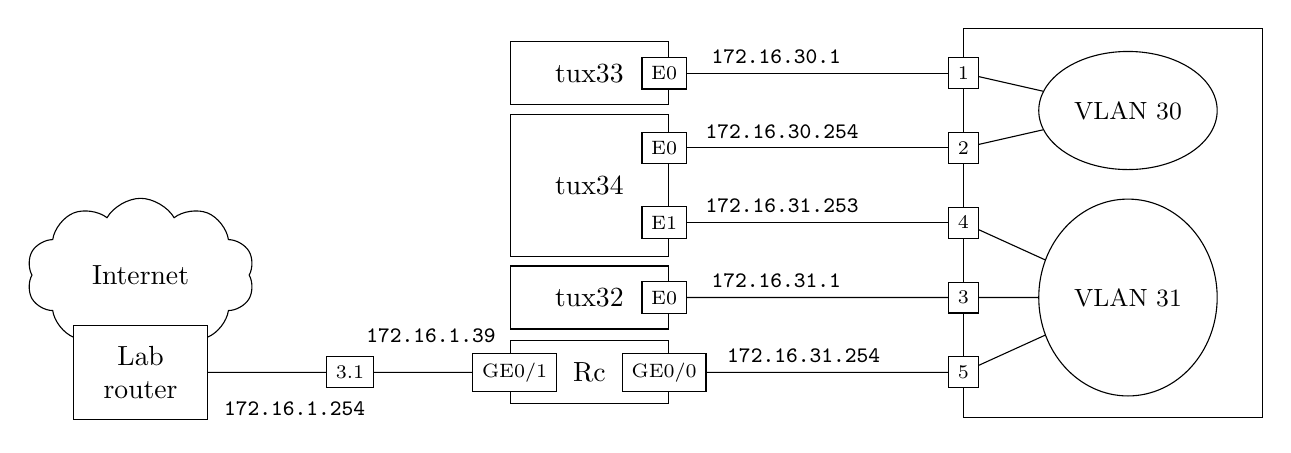
\begin{tikzpicture}[-,>=stealth',node distance=2cm,initial text=$ $,scale=0.95]
        \node at (0,-0) [rectangle,draw,minimum height=0.8cm, minimum width=2cm] (tux33) {tux33};
        \node at (1.0, -0) [rectangle, draw, fill=white] (tux33_E0){ \scriptsize E0 };

        \node at (0,-1.5) [rectangle,draw, minimum height=1.8cm, minimum width=2cm] (tux34) {tux34};
        \node at (1.0, -1) [rectangle, draw, fill=white] (tux34_E0){ \scriptsize E0 };
        \node at (1.0, -2) [rectangle, draw, fill=white] (tux34_E1){ \scriptsize E1 };
        
        \node at (0,-3) [rectangle,draw, minimum height=0.8cm, minimum width=2cm] (tux32) {tux32};
        \node at (1.0, -3) [rectangle, draw, fill=white] (tux32_E0){ \scriptsize E0 };

        \node at (0,-4) [rectangle,draw, minimum height=0.8cm, minimum width=2cm] (Rc) {Rc};
        \node at (1.0, -4) [rectangle, draw, fill=white] (Rc_GE0){ \scriptsize GE0/0 };
        \node at (-1.0, -4) [rectangle, draw, fill=white] (Rc_GE1){ \scriptsize GE0/1 };

        \node at (-3.2, -4) [rectangle, draw, fill=white] (3_1){ \scriptsize 3.1 };

        \node at (-6,-2.7) [cloud, draw,cloud puffs=10,cloud puff arc=120, aspect=1.8, inner ysep=1.2em] {Internet};
        \node at (-6,-4) [rectangle,draw, minimum height=1.2cm, minimum width=1.7cm, align=center, fill=white] (lab_router) {Lab\\router};

        \draw   (5, +0.6) rectangle ++(4, -5.2);
        \node at (7.2, -0.5) [ellipse, draw, minimum height = 1.5cm, minimum width = 2.0cm, align=center] (VLAN30) {\small VLAN 30};
        \node at (7.2, -3.0) [ellipse, draw, minimum height = 2.5cm, minimum width = 2.0cm, align=center] (VLAN31) {\small VLAN 31};
        \node at (5.0, -0.00) [rectangle, draw, fill=white] (switch_1){ \scriptsize 1 };
        \node at (5.0, -1.00) [rectangle, draw, fill=white] (switch_2){ \scriptsize 2 };
        \node at (5.0, -2.00) [rectangle, draw, fill=white] (switch_4){ \scriptsize 4 };
        \node at (5.0, -3.00) [rectangle, draw, fill=white] (switch_3){ \scriptsize 3 };
        \node at (5.0, -4.00) [rectangle, draw, fill=white] (switch_5){ \scriptsize 5 };

        \draw   (tux33_E0)    edge[above, align=left]     node[xshift=-0.45cm]{\footnotesize \texttt{172.16.30.1  }}          (switch_1)
                (tux34_E0)    edge[above, align=left]     node[xshift=-0.45cm]{\footnotesize \texttt{172.16.30.254}}          (switch_2)
                (tux32_E0)    edge[above, align=left]     node[xshift=-0.45cm]{\footnotesize \texttt{172.16.31.1  }}          (switch_3)
                (tux34_E1)    edge[above, align=left]     node[xshift=-0.45cm]{\footnotesize \texttt{172.16.31.253}}          (switch_4)
                (Rc_GE0)      edge[above, align=left]     node[xshift=-0.30cm]{\footnotesize \texttt{172.16.31.254}}          (switch_5)
                (Rc_GE1)      edge[above, align=right]    node[xshift=+0.10cm, yshift=+0.25cm]{\footnotesize \texttt{172.16.1.39}}            (3_1)
                (3_1)         edge[below, align=left]     node[xshift=+0.35cm, yshift=-0.25cm]{\footnotesize \texttt{172.16.1.254}}          (lab_router)

                (switch_1) edge[] (VLAN30)
                (switch_2) edge[] (VLAN30)
                (switch_3) edge[] (VLAN31)
                (switch_4) edge[] (VLAN31)
                (switch_5) edge[] (VLAN31)
            ;

    \end{tikzpicture}
	\caption{Network architecture for experiment 4}
	\label{fig:network_exp4}
\end{figure}

\subsubsection{Objectives} \label{sec:Obj4}

Configure a commercial router and implement NAT.

\subsubsection{Main configuration commands} \label{sec:Com4}
\subsubsection{Logs analysis} \label{sec:Log4}

When running the ping command from tux32 to tux33 without redirects, the packets first arrived on the router and then were redirected to tux34 and after it tux33.
After enabling the redirects and running ping again, the router sends a ICMP redirect message to tux32 that allows tux32 to directly send packets to tux34, without needing to go first through the router.

NAT is a method to translate IP addresses of computers in a network to a single public IP address.

\subsection{Experiment 5} \label{sec:Exp5}
\subsubsection{Objectives} \label{sec:Obj5}
Configure DNS
\subsubsection{Main configuration commands} \label{sec:Com5}
\begin{tabular}{p{11mm} | p{26mm} | p{112mm}}
    \textbf{Dev.} & \textbf{Description}                                  & \textbf{Commands}                       \\ \hline
    tux32, tux33, tux34      & Configure DNS & 
    \begin{lstlisting}[frame=none, numbers=none, language=sh, aboveskip=-0.5 \baselineskip, belowskip=-0.8 \baselineskip]
echo -e "search netlab.fe.up.pt\nnameserver 172.16.1.1" > /etc/resolv.conf
    \end{lstlisting}
\end{tabular}
\subsubsection{Logs analysis} \label{sec:Log5}

\subsection{Experiment 6} \label{sec:Exp6}
\subsubsection{Objectives} \label{sec:Obj6}
\subsubsection{Main configuration commands} \label{sec:Com6}
\subsubsection{Logs analysis} \label{sec:Log6}

\section*{Conclusion} \label{sec:Conclusion}

\bibliographystyle{acm}
\addcontentsline{toc}{section}{Bibliography}
\bibliography{report}

\appendix
\appendixpage
\addappheadtotoc
\chapter{Source code}

The source code of this project can be obtained from \href{https://github.com/dmfrodrigues/feup-rcom-l2}{github.com/dmfrodrigues/feup-rcom-l2}.
The source code is made available by \textcopyright~Diogo Rodrigues and Breno Pimentel under the \href{https://www.gnu.org/licenses/gpl-3.0.en.html}{GNU General Public License v3} (GPLv3), which you should have received together with the source code, or that you can otherwise obtain online.

During project development and evaluation the repository remained private, although it can be shared with evaluators on request to clarify the development process or due to other justifiable reasons.
It will be made public once all equivalent curricular unit projects have been evaluated in the present school year.

\newgeometry{top=24mm,bottom=24mm,left=14mm,right=14mm}
\fancyhfoffset{0pt}

\lstinputlisting[basicstyle=\ttfamily\small, caption=\texttt{url\_parser.h}, language=C]{../../download/include/url_parser.h}
\lstinputlisting[basicstyle=\ttfamily\small, caption=\texttt{url\_parser.c}, language=C]{../../download/src/url_parser.c}

\lstinputlisting[basicstyle=\ttfamily\small, caption=\texttt{server\_cmds.h}, language=C]{../../download/include/server_cmds.h}
\lstinputlisting[basicstyle=\ttfamily\small, caption=\texttt{server\_cmds.c}, language=C]{../../download/src/server_cmds.c}

\lstinputlisting[basicstyle=\ttfamily\small, caption=\texttt{download.h}, language=C]{../../download/include/download.h}
\lstinputlisting[basicstyle=\ttfamily\small, caption=\texttt{download.c}, language=C]{../../download/src/download.c}

\restoregeometry

\chapter{Configuration commands}
\lstinputlisting[basicstyle=\ttfamily\small, caption=\texttt{tuxy2\_config.sh}, language=bash]{../../part2/config/tuxy2_config.sh}
\lstinputlisting[basicstyle=\ttfamily\small, caption=\texttt{tuxy3\_config.sh}, language=bash]{../../part2/config/tuxy3_config.sh}
\lstinputlisting[basicstyle=\ttfamily\small, caption=\texttt{tuxy4\_config.sh}, language=bash]{../../part2/config/tuxy4_config.sh}
\lstinputlisting[basicstyle=\ttfamily\small, caption=\texttt{switch.sh}, language=cisco]{../../part2/config/switch.sh}
\lstinputlisting[basicstyle=\ttfamily\small, caption=\texttt{router.sh}, language=cisco]{../../part2/config/router.sh}

\newgeometry{top=24mm,bottom=24mm,left=14mm,right=14mm}
\fancyhfoffset{0pt}
\chapter{Logs}

\counterwithin{lstlisting}{subsection}
\renewcommand{\thelstlisting}{%
  \thechapter.\thesubsection(\arabic{lstlisting})%
}

\begin{center}
    \begin{tabular}{l | l | l}
        \textbf{Interface} & \textbf{MAC address}       & \texttt{IP address}    \\ \hline
        tux32-eth0         & \texttt{00:21:5a:61:30:63} & \texttt{172.16.31.1  } \\
        tux33-eth0         & \texttt{00:21:5a:61:24:92} & \texttt{172.16.30.1  } \\
        tux34-eth0         & \texttt{00:21:5a:5a:7d:74} & \texttt{172.16.30.254} \\
        tux34-eth2         & \texttt{00:c0:df:25:26:0a} & \texttt{172.16.31.253} \\
        Rc-GE0/0           & \texttt{                 } & \texttt{172.16.31.254} \\
        Rc-GE0/1           & \texttt{                 } & \texttt{172.16.1.39  } \\
    \end{tabular}
\end{center}

\section{Experiment 1}
\setcounter{subsection}{4}
\subsection{Item 5}
\lstinputlisting[basicstyle=\linespread{0.85}\ttfamily\small, frame=tbr, caption=\texttt{1-5-tux33-routes.txt}]{../../part2/exp1/1-5-tux33-routes.txt}
\lstinputlisting[basicstyle=\linespread{0.85}\ttfamily\small, frame=tbr, caption=\texttt{1-5-tux33-arp.txt}   ]{../../part2/exp1/1-5-tux33-arp.txt}
\lstinputlisting[basicstyle=\linespread{0.85}\ttfamily\small, frame=tbr, caption=\texttt{1-5-tux34-routes.txt}]{../../part2/exp1/1-5-tux34-routes.txt}
\lstinputlisting[basicstyle=\linespread{0.85}\ttfamily\small, frame=tbr, caption=\texttt{1-5-tux34-arp.txt}   ]{../../part2/exp1/1-5-tux34-arp.txt}

\begin{landscape}
\setcounter{subsection}{9}
\subsection{Item 10}
\lstinputlisting[basicstyle=\linespread{0.85}\ttfamily\scriptsize, frame=tbr, caption=\texttt{1-10-tux33.pcapng.txt}]{../../part2/exp1/1-10-tux33.pcapng.txt}
\end{landscape}

\begin{landscape}
\section{Experiment 2}

\setcounter{subsection}{4}
\subsection{Item 5}
\lstinputlisting[basicstyle=\linespread{0.85}\ttfamily\scriptsize, frame=tbr, caption=\texttt{2-5-tux33.pcapng.txt}]{../../part2/exp2/2-5-tux33.pcapng.txt} \pagebreak

\setcounter{subsection}{6}
\subsection{Item 7}

\lstinputlisting[basicstyle=\linespread{0.85}\ttfamily\scriptsize, frame=tbr, caption=\texttt{2-7-tux32.pcapng.txt}]{../../part2/exp2/2-7-tux32.pcapng.txt} \pagebreak
\lstinputlisting[basicstyle=\linespread{0.85}\ttfamily\scriptsize, frame=tbr, caption=\texttt{2-7-tux33.pcapng.txt}]{../../part2/exp2/2-7-tux33.pcapng.txt} \pagebreak
\lstinputlisting[basicstyle=\linespread{0.85}\ttfamily\scriptsize, frame=tbr, caption=\texttt{2-7-tux34.pcapng.txt}]{../../part2/exp2/2-7-tux34.pcapng.txt} \pagebreak

\setcounter{subsection}{9}
\subsection{Item 10}

\lstinputlisting[basicstyle=\linespread{0.85}\ttfamily\scriptsize, frame=tbr, caption=\texttt{2-10-tux32.pcapng.txt}]{../../part2/exp2/2-10-tux32.pcapng.txt} \pagebreak
\lstinputlisting[basicstyle=\linespread{0.85}\ttfamily\scriptsize, frame=tbr, caption=\texttt{2-10-tux33.pcapng.txt}]{../../part2/exp2/2-10-tux33.pcapng.txt} \pagebreak
\lstinputlisting[basicstyle=\linespread{0.85}\ttfamily\scriptsize, frame=tbr, caption=\texttt{2-10-tux34.pcapng.txt}]{../../part2/exp2/2-10-tux34.pcapng.txt}
\end{landscape}

\begin{landscape}
\section{Experiment 3}

\setcounter{subsection}{2}
\subsection{Item 3}
\lstinputlisting[basicstyle=\linespread{0.85}\ttfamily\small, frame=tbr, caption=\texttt{3-7-tux32.route.txt}]{../../part2/exp3/3-4-tux32.route.txt}
\lstinputlisting[basicstyle=\linespread{0.85}\ttfamily\small, frame=tbr, caption=\texttt{3-7-tux33.route.txt}]{../../part2/exp3/3-4-tux33.route.txt}
\lstinputlisting[basicstyle=\linespread{0.85}\ttfamily\small, frame=tbr, caption=\texttt{3-7-tux34.route.txt}]{../../part2/exp3/3-4-tux34.route.txt}

\setcounter{subsection}{6}
\subsection{Item 7}

\lstinputlisting[basicstyle=\linespread{0.85}\ttfamily\scriptsize, frame=tbr, caption=\texttt{3-7-tux33.pcapng.txt}]{../../part2/exp3/3-7-tux33.pcapng.txt} \pagebreak

\setcounter{subsection}{7}
\subsection{Item 8}

\lstinputlisting[basicstyle=\linespread{0.85}\ttfamily\scriptsize, frame=tbr, caption=\texttt{3-8-tux34-eth0.pcapng.txt}]{../../part2/exp3/3-8-tux34-eth0.pcapng.txt} \pagebreak
\lstinputlisting[basicstyle=\linespread{0.85}\ttfamily\scriptsize, frame=tbr, caption=\texttt{3-8-tux34-eth1.pcapng.txt}]{../../part2/exp3/3-8-tux34-eth1.pcapng.txt}
\end{landscape}


\section{Experiment 4}

\setcounter{subsection}{2}
\subsection{Item 3}
\lstinputlisting[basicstyle=\linespread{0.85}\ttfamily\scriptsize, frame=tbr, caption=\texttt{4-3-tux33.pcapng.txt}]{../../part2/exp4/4-3-tux33.pcapng.txt}

\setcounter{subsection}{3}
\subsection{Item 4}
                 \lstinputlisting[basicstyle=\linespread{0.85}\ttfamily\small     , frame=tbr, caption=\texttt{4-4c-tux32-noredirect-noroute.ping.txt}       ]{../../part2/exp4/4-4c-tux32-noredirect-noroute.ping.txt}
\begin{landscape}\lstinputlisting[basicstyle=\linespread{0.85}\ttfamily\scriptsize, frame=tbr, caption=\texttt{4-4c-tux32-noredirect-noroute.pcapng.txt}     ]{../../part2/exp4/4-4c-tux32-noredirect-noroute.pcapng.txt}\end{landscape}
                 \lstinputlisting[basicstyle=\linespread{0.85}\ttfamily\small     , frame=tbr, caption=\texttt{4-4e-tux32-noredirect-noroute.traceroute.txt} ]{../../part2/exp4/4-4e-tux32-noredirect-noroute.traceroute.txt}
                 \lstinputlisting[basicstyle=\linespread{0.85}\ttfamily\small     , frame=tbr, caption=\texttt{4-4f-tux32-noredirect-yesroute.traceroute.txt}]{../../part2/exp4/4-4f-tux32-noredirect-yesroute.traceroute.txt}
                 \lstinputlisting[basicstyle=\linespread{0.85}\ttfamily\small     , frame=tbr, caption=\texttt{4-4g-tux32-yesredirect-noroute.ping.txt}      ]{../../part2/exp4/4-4g-tux32-yesredirect-noroute.ping.txt}
\begin{landscape}\lstinputlisting[basicstyle=\linespread{0.85}\ttfamily\scriptsize, frame=tbr, caption=\texttt{4-4g-tux32-yesredirect-noroute.pcapng.txt}    ]{../../part2/exp4/4-4g-tux32-yesredirect-noroute.pcapng.txt}\end{landscape}

\setcounter{subsection}{4}
\subsection{Item 5}
                 \lstinputlisting[basicstyle=\linespread{0.85}\ttfamily\small     , frame=tbr, caption=\texttt{4-5-tux33.ping.txt}  ]{../../part2/exp4/4-5-tux33.ping.txt}
\begin{landscape}\lstinputlisting[basicstyle=\linespread{0.85}\ttfamily\scriptsize, frame=tbr, caption=\texttt{4-5-tux33.pcapng.txt}]{../../part2/exp4/4-5-tux33.pcapng.txt}\end{landscape}

\setcounter{subsection}{6}
\subsection{Item 7}
                 \lstinputlisting[basicstyle=\linespread{0.85}\ttfamily\small     , frame=tbr, caption=\texttt{4-7-tux33.ping.txt}  ]{../../part2/exp4/4-7-tux33.ping.txt}
\begin{landscape}\lstinputlisting[basicstyle=\linespread{0.85}\ttfamily\scriptsize, frame=tbr, caption=\texttt{4-7-tux33.pcapng.txt}]{../../part2/exp4/4-7-tux33.pcapng.txt}\end{landscape}

\section{Experiment 5}
\setcounter{subsection}{2}
\subsection{Item 3}
                 \lstinputlisting[basicstyle=\linespread{0.85}\ttfamily\small     , frame=tbr, caption=\texttt{5-3-tux33.ping.txt}  ]{../../part2/exp5/5-3-tux33.ping.txt}
\begin{landscape}\lstinputlisting[basicstyle=\linespread{0.85}\ttfamily\scriptsize, frame=tbr, caption=\texttt{5-3-tux33.pcapng.txt}]{../../part2/exp5/5-3-tux33.pcapng.txt}\end{landscape}

\section{Experiment 6}

\setcounter{subsection}{1}
\subsection{Item 2}
\subsubsection{Transferring \texttt{pipe.txt}}
                 \lstinputlisting[basicstyle=\linespread{0.85}\ttfamily\small, frame=tbr, label={listing:6-2-tux33-pipe}, caption=\texttt{6-2-tux33-pipe.download.txt}]{../../part2/exp6/6-2-tux33-pipe.download.txt}
\begin{landscape}\lstinputlisting[basicstyle=\linespread{0.85}\ttfamily\tiny , frame=tbr,                                 caption=\texttt{6-2-tux33-pipe.pcapng.txt}  ]{../../part2/exp6/6-2-tux33-pipe.pcapng.txt}\end{landscape}

\subsubsection{Transferring \texttt{pic2.png}}
                 \lstinputlisting[basicstyle=\linespread{0.85}\ttfamily\small, frame=tbr, label={listing:6-2-tux33-pic2}, caption=\texttt{6-2-tux33-pic2.download.txt}]{../../part2/exp6/6-2-tux33-pic2.download.txt}
\begin{landscape}\lstinputlisting[basicstyle=\linespread{0.85}\ttfamily\tiny , frame=tbr,                                 caption=\texttt{6-2-tux33-pic2.pcapng.txt}  ]{../../part2/exp6/6-2-tux33-pic2.pcapng.txt}\end{landscape}

\setcounter{subsection}{4}
\subsection{Item 5}
                 \lstinputlisting[basicstyle=\linespread{0.85}\ttfamily\small, frame=tbr, label={listing:6-5-tux32}, caption=\texttt{6-5-tux32.download.txt}]{../../part2/exp6/6-5-tux32.download.txt}
\begin{landscape}\lstinputlisting[basicstyle=\linespread{0.85}\ttfamily\tiny , frame=tbr,                            caption=\texttt{6-5-tux32.pcapng.txt}  ]{../../part2/exp6/6-5-tux32.pcapng.txt}\end{landscape}
                 \lstinputlisting[basicstyle=\linespread{0.85}\ttfamily\small, frame=tbr, label={listing:6-5-tux33}, caption=\texttt{6-5-tux33.download.txt}]{../../part2/exp6/6-5-tux33.download.txt}
\begin{landscape}\lstinputlisting[basicstyle=\linespread{0.85}\ttfamily\tiny , frame=tbr,                            caption=\texttt{6-5-tux33.pcapng.txt}  ]{../../part2/exp6/6-5-tux33.pcapng.txt}\end{landscape}

\restoregeometry

\end{document}
